\chapter{\IfLanguageName{dutch}{Stand van zaken}{State of the art}}
\label{ch:stand-van-zaken}

% Tip: Begin elk hoofdstuk met een paragraaf inleiding die beschrijft hoe
% dit hoofdstuk past binnen het geheel van de bachelorproef. Geef in het
% bijzonder aan wat de link is met het vorige en volgende hoofdstuk.

% Pas na deze inleidende paragraaf komt de eerste sectiehoofding.

Dit onderzoek heeft als doel om, uit drie kandidaten, één end-to-end testing framework aan te duiden dat het meest geschikt is voor de use case van Colruyt Group, zoals beschreven in het voorgaande hoofdstuk. Deze drie kandidaat-frameworks zijn de volgende:

\begin{enumerate}
    \item Protractor
    \item Cypress
    \item UFT
\end{enumerate}

In dit hoofdstuk worden eerst de principes van een robuuste testarchitectuur besproken. Dit om de nodige context te geven voor de drie kandidaat-frameworks, die daarna besproken worden. Ten slotte worden drie zogeheten ``Behavior Driven Development'' (BDD) frameworks onder de loep genomen. Deze frameworks zijn een extra laag bovenop een testing framework en maken het mogelijk acceptatietesten in quasi natuurlijke taal te schrijven, wat de implementatie versnelt (\cite{Diepenbeck2014}).

\section{Testing Architectuur}

De consensus is dat grofweg 50\% van de middelen van een softwareproject besteed worden aan de testfase \cite{Kasurinen2010,Tsai2001,Dadwal2018}. Er is met andere woorden een sterk (financieel) motief om dit aandeel te verkleinen middels test automatisatie.

Wie het implementeren van test automatisatie overweegt, dient er zich bewust van te zijn dat de kosten daarvan hoger zijn tijdens de eerste release van het test automatisatiesysteem \autocite{Fewster2001} \autocite{Kumar2016}. Dit is althans het geval wanneer men een minimale onderhoudskost nastreeft. In dit geval kunnen de kosten geassocieerd met test automatisatie op \emph{lange} termijn echter gereduceerd worden tot minder dan de helft van de kost om het testen 100\% manueel uit te voeren \autocite{Kumar2016}.

Een bijkomend voordeel is dat de vrijgekomen tijd bij het testing team gebruikt kan worden voor de meest complexe en veeleisende test cases (\cite{Barrett2013}).

Eerder onderzoek door Persson en Yilmaztürk wees uit dat de onderhoudbaarheid van een test automatisatiesysteem ondergeschikt maken aan het gemak van implementatie een groter risico op falen met zich meebrengt \autocite{Persson2004}. Een weloverwogen testarchitectuur is met andere woorden onontbeerlijk voor het slagen van een test automatisatiesysteem. Sterker nog: het ontwikkelingsproces van een test automatisatiesysteem zou vrijwel analoog moeten zijn aan dat van de eigenlijke software \autocite{Pettichord1996}.

\subsection{Multitierarchitectuur}

Bij het ontwikkelen van software volgens de Agile filosofie is het noodzakelijk (geautomatiseerde) test cases continu te herwerken om ze representatief te houden \autocite{Day2014}. Een test automatisatiesysteem dat gebaseerd is op een multitierarchitectuur (ook: n-tier architectuur) kan de onderhoudskosten desondanks relatief laag houden.

Concreet zal een multitierarchitectuur de verschillende soorten functionaliteit uit elkaar halen en los van elkaar testen. Idealiter zou elk van de lagen van de software vervangen moeten kunnen worden door één van de test automatisatielagen zonder hierdoor fouten of onverwacht gedrag te introduceren \autocite{Anandan}. Day stelt zelf 4 standaardtiers voor:

\begin{enumerate}
    \item ``Presentation'': de grafische interface en gebruikerservaring, die vaak middels \emph{smoke style testing}\footnote{\textbf{Smoke testing} focust zich op een handvol eenvoudige testen om de meest voor de hand liggende scenario's te valideren en zware fouten er uit te halen \autocite{Klostermann2019}.} gevalideerd wordt
    \item ``Business'': domeinlogica, die in de meeste gevallen het grootste aandeel te testen functionaliteit vertegenwoordigd
    \item ``Data'': opslag en ophalen van gegevens
    \item ``Web Services''
\end{enumerate}

De tiers kunnen evengoed georganizeerd worden in een \emph{front-end} (de grafische gebruikersomgeving) en een \emph{back-end} (logica, data en services) view, zoals ook Day doet in zijn case study.

\subsection{End-to-End Testing}

Een mulitierarchitectuur laat toe softwaremodules in afzondering te valideren, wat het mogelijk maakt fouten snel en met grote nauwkeurigheid te identificeren. Om te kunnen stellen dat een gegeven softwareproduct aan de vooropgestelde kwaliteitseisen voldoet, moet dat product echter ook als een geheel én in zijn gebruikscontext gevalideerd worden. Dit gebeurt hoofdzakelijk op twee manieren \cite{Tsai2001}:

\begin{enumerate}
    \item ``Integratietesting'': test meerdere modules als groep (subsysteem) 
    \item ``End-to-End (E2E) (integratie)testing'': testen van de functionaliteit van een applicatie vanuit een \textbf{gebruikersstandpunt}, vindt normaliter plaats na de integratietesting
\end{enumerate}

\subsubsection{Thin Threads}

Tsai et al. stellen in hun paper van 2001 een aanpak voor het ontwerpen van E2E testingsystemen voor die zich focust op zogeheten ``\textbf{thin threads}''. Elke thin-thread vertegenwoordigd één gebruikersscenario, heeft een aantal voorwaarden (``condities'') en kent eventueel input- en/of outputgegevens. \textbf{Condities} kunnen te maken hebben met gegevens (verplichtheid van en vereisten gesteld aan de data), communicatie (time-outs en recovery mechanismen, security), de volgorde van operaties (coördinatie, updates) of eventuele andere factoren.

Zowel thin-threads als hun condities hebben onderlinge relaties en kunnen in een boomstructuur georganiseerd worden.

\begin{figure}[h!]
    \centering
    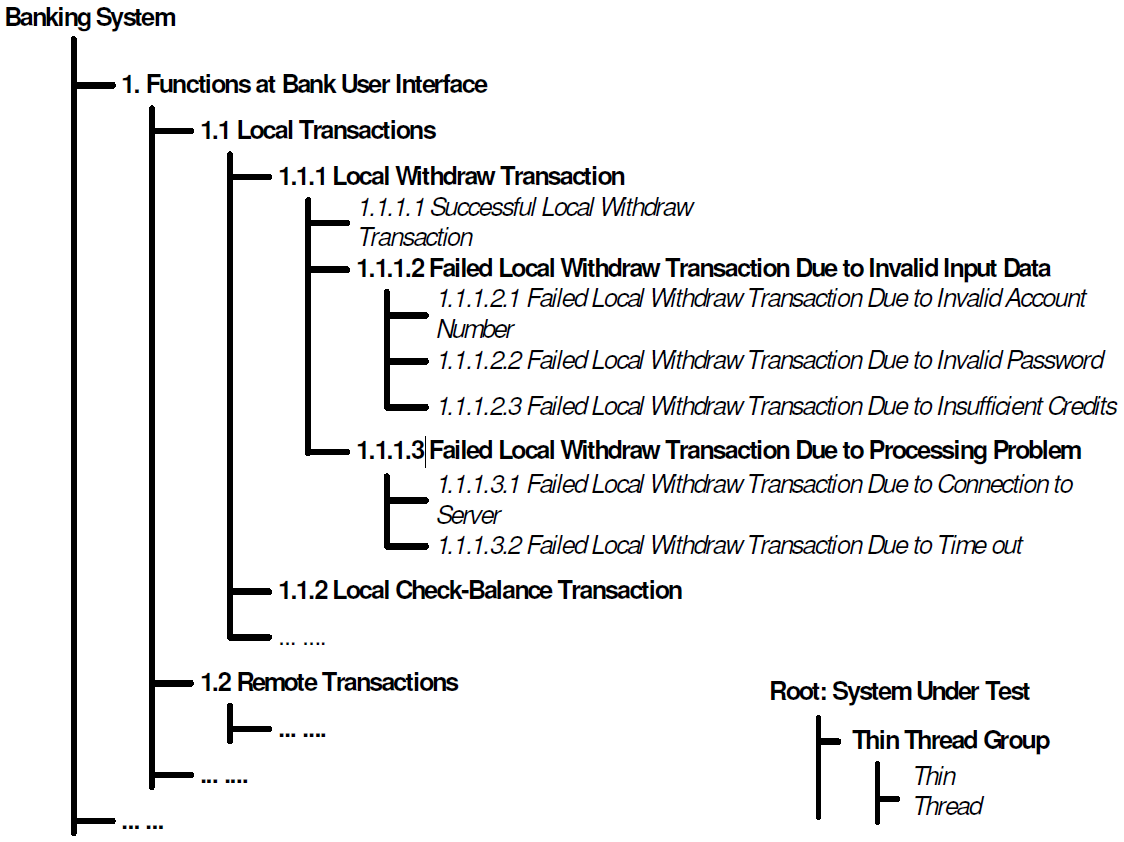
\includegraphics[scale=0.45]{img/Tsai2001ThinThreadTree.png}
    \caption{Een hypothetische thin-thread boom voor een bankiersapplicatie ~\cite{Tsai2001}}
    \label{fig:tsaithinthreadtree}
\end{figure}

De relaties tussen thin-threads onderling worden bepaald door hoe hun uitvoeringspaden zich tot elkaar verhouden:

\begin{enumerate}
    \item ``Deel-geheel'': het pad van één thin-thread is deel van dat van een andere thin-thread
    \item ``Identiek'': de paden zijn identiek; ze delen condities of andere eigenschappen
    \item ``Onafhankelijk'': de thin-threads hebben volledig andere paden
\end{enumerate}

Ook de condities kennen een reeks mogelijke verhoudingen:

\begin{enumerate}
    \item ``Onafhankelijk'': één conditie kan zich met of zonder een andere voordoen
    \item ``Gekoppeld'': één conditie kan of zal de andere veroorzaken
    \item ``Wederzijds uitgesloten'': slechts één van beide kan zich in één situatie voordoen
    \item ``Gerelateerd'': twee condities worden in dezelfde thin-thread gebruikt of sluiten elkaar uit
\end{enumerate}

Bij het opstellen van \textbf{E2E test cases} op basis van deze techniek dienen eerst de de thin-threads, hun condities, hun mogelijke input- en outputgegevens, en de relaties tussen de thin-threads en de condities onderling vastgelegd te worden. De test cases worden vervolgens opgebouwd uit individuele thin-threads. Thin-threads kunnen na elkaar uitgevoerd worden (``sequencing''), herhaald worden (``looping'') en op basis van voorwaarden uitgevoerd worden (``conditioned execution'').

\begin{figure}[h!]
    \centering
    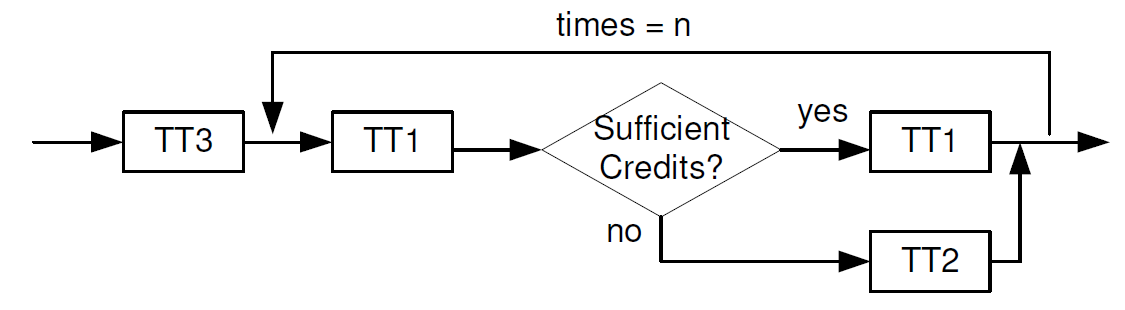
\includegraphics[scale=0.35]{img/Tsai2001ComplexTestScenario.png}
    \caption{Voorbeeld van een test case opgebouwd uit 3 verschillende thin-threads ~\cite{Tsai2001}}
    \label{fig:tsaicomplexscenario}
\end{figure}

Om de test cases te vervolledigen tot reële gebruiksscenario's moet men ten slotte inputs kiezen op basis van de grenzen van de condities. Meestal gaat men \emph{grenswaarden} kiezen om te testen \autocite{Jorgensen2013}, maar dit kan ook door: de input \emph{willekeurig} te selecteren \autocite{Loo1988}, de mogelijke inputs in \emph{categorieën} te sorteren en daar representatieve data uit halen of door eenvoudigweg data uit de reële gebruiksomgeving te gebruiken (\emph{``usage-based testing''}) \autocite{Dyer1992}.

\subsection{Overwegingen bij de Keuze voor een Test Automatisatiesysteem}

Test automatisatie vergt een substantiële initiële investering; analyse van de functionaliteit van de software, schrijven van testscripts, het introduceren van de tooling en het opleiden van personeel etc. \autocite{Kumar2016}. Het is dus van kritisch belang om een weloverwogen keuze te maken teneinde de kans op slagen van dergelijk project te maximaliseren. De volgende factoren zijn in het bijzonder belangrijk in acht te nemen:

\begin{itemize}
    \item \emph{De betrokken technologieën en omgevingen}. Het spreekt voor zich dat men voor het opzetten van test automatisatie anders te werk zal moeten gaan bij mainframe toepassingen dan voor webapplicaties. De beschikbare tooling zal ook afhankelijk zijn van de gebruikte technologieën (\cite{10.1145/1295014.1295062}).
    \item \emph{De beschikbare kennis}. Ervaring met een bepaald framework binnen het team is een sterke troef en vaak een doorslaggevende reden om een keuze te motiveren (\cite{Madan2013}).
    \item \emph{De lifecycle van de software}. Het te implementeren systeem dient te passen binnen het geplande levensverloop van de software zelf. Software waarvoor slechts een beperkt aantal toekomstige releases (of zelfs helemaal \emph{geen} toekomstige ontwikkeling) gepland is, zal niet gebaat zijn bij test automatisatie \autocite{Tiitinen2013}.
\end{itemize}

\section{e2e Testing Frameworks voor Angular}

\autocite{Anandan}
\autocite{Kumar2016}
\autocite{Barrett2013}
\autocite{Holmes}
\autocite{Singh2015}
\autocite{Madan2013}

\lipsum[4]

\subsection{Protractor}

\lipsum[6-7]

\subsection{Cypress}

\lipsum[3-4]

\subsection{UFT}

\lipsum[3-4]

\subsection{Behavior Driven Development Frameworks}

\lipsum[9]

\subsubsection{Mocha}

\lipsum[8-10]

\subsubsection{Jasmine \& Karma}

\lipsum[8-10]

\subsubsection{Cucumber}

\lipsum[8-10]